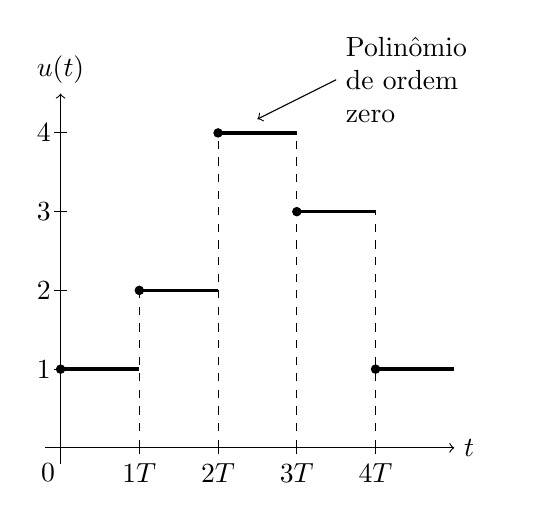
\begin{tikzpicture}
\draw[->] (-0.2,0) -- (5,0) node[right] {$t$};
\draw[->] (0,-0.2) -- (0,4.5) node[above] {$u(t)$};

\draw (0,0) ++(-0.16,-0.08) node[below] {$ 0 $};

\foreach \x in {1,...,4}{
	\draw (\x,0) ++(0,-0.08) node[below] {$ \x T $} -- +(0,.16);
	\node[left] at (0,\x) {$ \x $};
	\draw (0,\x) ++(-0.08,0) -- +(.16,0);
}

\draw[] plot[jump mark left, mark=*, mark size=1.5pt] coordinates{(0,1) (1,2) (2,4) (3,3) (4,1)};

\draw[line width=1.2pt] (0,1) -- (1,1) (1,2) -- (2,2) (2,4) -- (3,4) (3,3) -- (4,3) (4,1) -- (5,1);

\draw (4,1) -- +(0.8,0);

\draw[dashed] plot[ycomb, no marks] coordinates{(1,2) (2,4) (3,4) (4,3)};

\draw[<-] (2.5,4) ++(0,5pt) -- +(1,0.5) node[right,text width=2cm] {Polinômio de ordem zero};
\end{tikzpicture}